\documentclass[../thesis.tex]{subfiles}
\begin{document}

\section{data\_barrier Class} % (fold)

The motivation for the data\_barrier class is simple; in order to fully distribute OpenCL programming there needs to be some form of interconnection between the distributed systems. This is where the data\_barrier comes in, it is the point of connection between the multiple systems, and as such it was important to get it right. It is meant to essentially be a data barrier located between two or more machines, their point of interconnection. A visualization of the barrier can be seen in Figure~\ref{fig:data_barrier_vis}.

\begin{figure}[htbp]
  \centering
  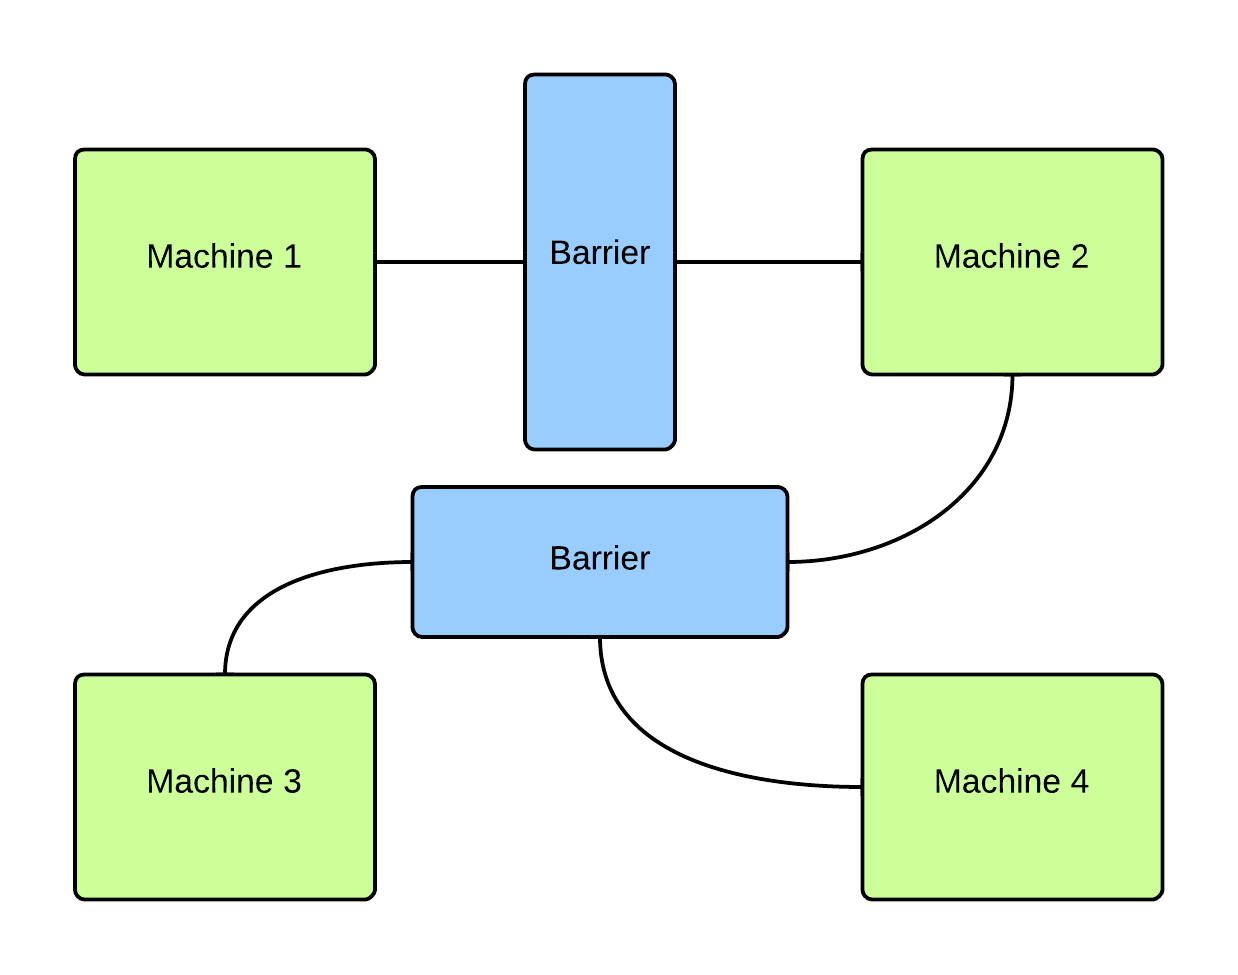
\includegraphics[width=0.95\textwidth]{diagrams/data_barrier_visual.png}
  \caption{Data Barrier Visualization}
  \label{fig:data_barrier_vis}
\end{figure}

In this, there is a shared barrier between Machine 1 and 2, and a shared barrier between Machines 2, 3, and 4. Thus data transfers between Machine 1 and 3/4 can only occur if they pass through Machine 2 first. That is what data barriers are for, points where data can pass through and be synchronized.

The class was meant to contain all the functions and information necessary for the transference of data between machines. The actual members can be seen in Figure~\ref{fig:data_barrier_class}, a UML diagram for the data\_barrier class.

\begin{figure}[htbp]
  \centering
  \includegraphics[width=0.95\textwidth]{diagrams/data_barrier_class.1}
  \caption{Data Barrier Class UML Diagram}
  \label{fig:data_barrier_class}
\end{figure}

The first aspect of the data\_barrier class that will be examined at are its data members. After looking into the various data members of the data\_barrier, as well as the motivations for each of them, all aspects of the member functions will be examined; their development from start to finish, their use, and future possible improvements.

\subsection{Data Members} % (fold)
\label{sub:data_members}
  The easiest way to gain an understanding of the data members is to look at the constructor for the data barrier, and then examine each component in turn. By looking at the required pieces to create a data\_barrier, we can see how they tie in with the underlying data members. As can be seen in Figure~\ref{fig:data_barrier_constructor}, there are quite a few variables that go into the creation of a data\_barrier, each will be examined in turn. However, prior to looking at these, we'll look at the first aspect of the constructor, the templating.

  \begin{figure}[htbp]
    \centering

    \lstset{language=cpp}  
    \begin{lstlisting}[tabsize=2]
template <typename data_type> data_barrier<data_type>::data_barrier(const init_list &machines, int size_x, int granularity, int tag_value, int id, cl_context input_context)
{
  data_size = size_x;
  if(data_size % granularity!= 0)
    std::runtime_error("Error, data_size % granularity must equal 0");
  number_chunks = size_x / granularity;
  chunk_size = granularity;
  message_tag = tag_value;
  machine_id = id;
  shared_machine_list = machines;
  data = new data_type[data_size];
  previous_data = new data_type[data_size];
  context = input_context;
}
      \end{lstlisting}

    \caption{data\_barrier Constructor}
    \label{fig:data_barrier_constructor}
  \end{figure}
   

  \subsubsection{template <typename data\_type>} % (fold)
  \label{ssub:template_typename_data_type}
    data\_barrier is, itself, a templated class. The motivation behind this is quite straightforward; reduce the amount of needless repetition of code. It would have been quite possible to write a different data\_barrier class for each of the possible OpenCL data\_types. Unfortunately, that would be a hugely wasteful use of time, the code would be practically the same for every single possible data\_type, with very minor variations. This would have led to an explosion of code; with more than ten possible data\_types \cite{opencldatatypes} in OpenCL 1.2, it made sense not to have so much duplication within the code. Thus data\_barrier was a templated class, and all it's internal functions are templated as well.

    In practice, this just means that during construction you must provide the data\_type you require, as opposed to using a different class on a per data type basis. This can be seen in Figure~\ref{fig:templated_vs_non_templated}, where a single templated class is shown in contrast with a set of non-templated classes to provide what is, in the end, the same result.

    \begin{figure}[htbp]
      \centering

      \lstset{language=cpp}  
      \begin{lstlisting}[tabsize=2]
//templated class for float and int barriers
data_barrier<float> float_barrier_templated = data_barrier<float>(machines, size_x, granularity, tag_value, id,  input_context);

data_barrier<int> int_barrier_templated = data_barrier<int>(machines, size_x, granularity, tag_value, id,  input_context);

//non templated classes for float and int barriers
float_data_barrier float_barrier = float_data_barrier(machines, size_x, granularity, tag_value, id,  input_context);

int_data_barrier int_barrier = int_data_barrier(machines, size_x, granularity, tag_value, id,  input_context);
        \end{lstlisting}

      \caption{The Difference Between Templated and Generic Classes}
      \label{fig:templated_vs_non_templated}
    \end{figure}
  % subsubsection template_typename_data_type (end)
  
  \subsubsection{init\_list \texttt{\&}machines} % (fold)
  \label{ssub:init_list}
    The next component of the constructor, and one of the most important, is the init\_list. Init\_list is simply a macro for \newline\texttt{std::initializer\_list<int> \&machines}, a templated standard C\texttt{++} class, in this case with type integer. The purpose behind it's use is readily apparent once seen; it is used to easily allow the programmer to declare a list of integers defining the machines that the data\_barrier will target.

    This is actually used quite frequently throughout the majority of code, and while it has it's own foibles in usage, the ability to provide a simple and quick inline declaration of targeted machines is quite useful. Its use can be seen in Figure~\ref{fig:init_list_vs_others}; which compares the use of a statically initialized array, a vector, and an initializer\_list.

     \begin{figure}[htbp]
      \centering

      \lstset{language=cpp}  
      \begin{lstlisting}[tabsize=2]
// Functions for each data type
void arrayFunc(int array[]){};
void vectorFunc(std::vector<int> vec){};
void initlistFunc(std::initializer_list<int> &initlist){};

// An array
int myArray[3] = {1,2,4};
arrayFunc(myArray);

// A vector (inline declaration allowed as of C++11)
std::vector<int> vec = {1, 2, 4};
vectorFunc(vec);

// initializer_list
initlistFunc({1,2,4});
        \end{lstlisting}

      \caption{Initalizer Lists vs Arrays and Vectors}
      \label{fig:init_list_vs_others}
    \end{figure}

    Although this ignores how the data passed in is handled, from the perspective of someone using this library, that is not important. As such, the use of an initializer\_list allows for an inline declaration, easing the burden on the programmer.

    As for what this is actually used for, as mentioned briefly above it is a list of the machines that are targeted by the data\_barrier. What that means in this context, is that if the machine is not contained within the list, any machines that use this barrier in a function call immediately return having done nothing. Additionally, and this is covered later, there is a factory function that returns an empty class object if not one of the target machines.

    The value `machines' is stored within the data member shared\_machine\_list, which is used by many functions to quickly check if the machine listed is valid to be targeted by a function call.
  % subsubsection init_list (end)

  \subsubsection{int size\_x} % (fold)
  \label{ssub:int_size_x}
      The next component in the constructor is size\_x. As can be seen in Figure~\ref{fig:data_barrier_constructor}, size\_x is used in three data members; \texttt{data\_type * data}, \texttt{int data\_size}, and \texttt{int number\_chunks}.

      The data\_size member is quite straightforward; it is the number of values contained within \texttt{data\_type * data}. In this situation, its value is a quite straightforward assignment from size\_x to data\_size, because it is dealing with a one dimensional array. Given a greater dimensional array, more values would be included in the constructor (such as size\_y and size\_z), but for this one-dimensional array only one is needed.

      This leads directly to \texttt{data\_type * data}, an array of data\_type of data\_size. This is, quite obviously, the most important component of the data\_barrier, for it is the actual data that is dealt with.

      Additionally, there is \texttt{data\_type * previous\_data}, an array of size data\_size used for determining what data needs to be sent during a synchronization event.
  % subsubsection int_size_x (end)

  \subsubsection{int granularity} % (fold)
  \label{ssub:int_granularity}
    Granularity follows very closely on \texttt{int data\_size}'s heels; it determines the granularity with which data transfers are correct to. It essentially divides \texttt{data\_type * data} into a series of chunks of a given size, which is stored within data\_barrier as \texttt{int chunk\_size}.

    Whenever data is transfered between machines, it is done so in these chunks, and the atomicity of these transactions is guaranteed. Thus if two machines are simultaneously sending data to a third, there is a guarantee that data will be correct on a per chunk basis, although if both machines are sending the same chunk there is no guarantee which chunk will be kept.

    Finally, the granularity is used in conjunction with data\_size to determine another data member, \texttt{int number\_chunks}. This is quite straightforward as well, the number of chunks of size granularity that fit within data\_size. One restriction upon these, is that \texttt{data\_size \% granularity == 0}.

    That is to say, the number of chunks multiplied by the size of the chunks must be equal to the size of the data. If the chunks do not perfectly align, an error will be thrown.
 
    As seen in Figure~\ref{fig:data_transfer_chunk_guarantee}, granularity is useful when multiple machines are manipulating a single data\_barrier. In this situation, we have an array of size 4 with a granularity of 2, that is the data is viewed as two discrete chunks. In Cycle1, Machine1 changes the lower half of the data, while Machine3 simultaneously changes the upper half. When data is transfered to Machine2 in Cycle2, there is no conflict between the data that is exchanged; and so Machine2's data ends up as expected.

    However, in Cycle3, both Machine1 and Machine3 modify all their data. When they transfer that data to Machine2 in Cycle4, there is a conflict; and so the upper half of the data may be either D D or F F, and the bottom half may also be either D D or F F. Were the granularity of this data barrier changed to a granularity of 1, each node in the array would be sent by itself. In Cycle2 there would be no change; the machines still operated on a unique chunks of data. In Cycle4, however, the data could be any combination of D and F. By keeping data in chunks, when synchronizing the machines, you can guarantee that as long as any given chunk was modified by only one machine, there will be no conflict in that chunk of data.

    \begin{figure}[htbp]
      \centering
      \tikzset{my arrow/.style={blue!60!black,-latex}}
      \tikzset{transfer arrow/.style={blue!60!black,->,out=-90, in=90}}
      \tikzset{transfer arrow left/.style={red!60!black,->,out=-50, in=130}}
      \tikzset{transfer arrow right/.style={green!60!black,->,out=-130, in=50}}

      \begin{tikzpicture}
        \matrix[matrix of math nodes, row sep=4mm] (M)
        {
         \node{Cycle 0}; & \node {[A A}; &[-1mm] \node{A A]}; &[10mm] \node  {[A A}; &[-1mm] \node{A A]};  &[10mm] \node {[A A}; &[-1mm] \node{A A]}; \\ 
          \node{Cycle 1}; & \node {[B B}; & \node{A A]}; & \node {[A A}; & \node{A A]};  & \node {[A A}; & \node{C C]}; \\
          \\
          \node{Cycle 2}; & \node {[B B}; & \node{A A]}; & \node {[B B}; & \node{C C]};  & \node {[A A}; & \node{C C]}; \\ 
          \node{Cycle 3}; & \node {[D D}; & \node{D D]}; & \node {[B B}; & \node{C C]};  & \node {[F F}; & \node{F F]}; \\
          \\
          \node{Cycle 4}; & \node {[D D}; & \node{D D]}; & \node {[X X}; & \node{Y Y]};  & \node {[F F}; & \node{F F]}; \\  
        };
        \node [above, xshift=4mm] at (M-1-2.north) {Machine 1};
        \node [above, xshift=4mm] at (M-1-4.north) {Machine 2};
        \node [above, xshift=4mm] at (M-1-6.north) {Machine 3};

        \draw[my arrow] (M-1-2) to (M-2-2);
        \draw[my arrow] (M-1-7) to (M-2-7);
        \draw[transfer arrow] (M-2-2) to (M-4-4);
        \draw[transfer arrow] (M-2-7) to (M-4-5);
        \draw[my arrow] (M-4-2) to (M-5-2);
        \draw[my arrow] (M-4-3) to (M-5-3);
        \draw[my arrow] (M-4-6) to (M-5-6);
        \draw[my arrow] (M-4-7) to (M-5-7);
        \draw[transfer arrow left] (M-5-2) to (M-7-4);
        \draw[transfer arrow left] (M-5-3) to (M-7-5);
        \draw[transfer arrow right] (M-5-6) to (M-7-4);
        \draw[transfer arrow right] (M-5-7) to (M-7-5);
      \end{tikzpicture}


      \caption{Data Transfer Granularity Assurance}
      \label{fig:data_transfer_chunk_guarantee}
      \end{figure}

      It should be noted, however, that there is a limitation to the amount of granularity available. The graph in Figure~\ref{fig:message_overhead} was produced by Douglas Doerfler and Ron Brightwell in their paper ``Measuring MPI Send and Receive Overhead and Application Availability in High Performance Network Interfaces'' \cite{mpioverhead}.

      \begin{figure}[htbp]
        \centering
        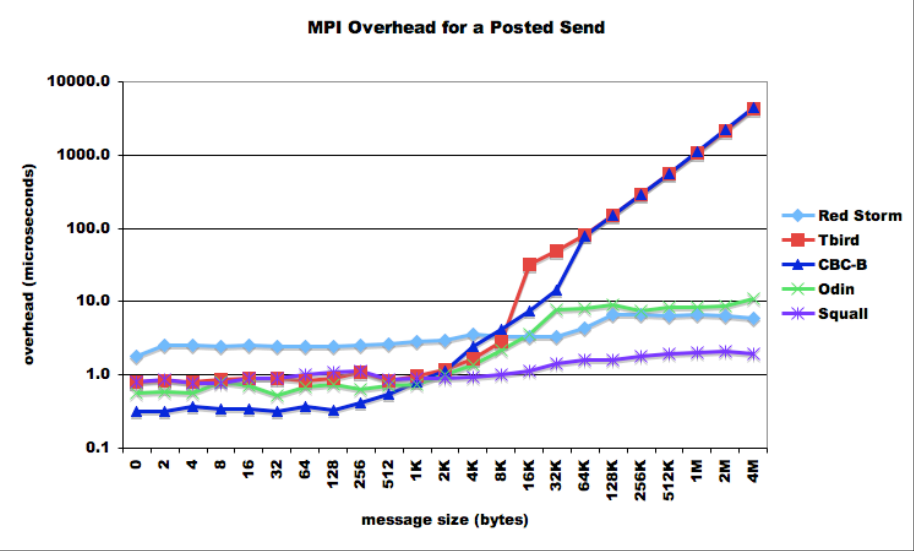
\includegraphics[width=0.95\textwidth]{diagrams/message_overhead.png}
        \caption{MPI Message Overhead}
        \label{fig:message_overhead}
      \end{figure}

    In it you can see the overhead required for an Isend for various test platforms. Although non of these applications utilize OpenMPI as their MPI distribution, whereas my project does, the point still stands that sending data can incur a significant overhead. For the most part, it seems best to aim for a chunk size of 8 kilobytes, where you achieve the best balance between overhead and data sent. In future work, validating these expectations experimentally would be worthwhile.
  % subsubsection int_granularity (end)

  \subsubsection{int tag\_value} % (fold)
  \label{ssub:int_tag_value}
    Tag\_value has a relatively straightforward usage; it provides a tag so that there are no collisions between messages. OpenMPI is used for data transfers, and one of the parameters for sending messages is the message tag. By assigning a unique value to message\_tag via tag\_value, we can assure that there will be no collisions between messages from different data\_barriers. Choosing the tag\_value is actually hidden away from the user by the distributedCL class, however there will be more discussion on that later.
  % subsubsection int_tag_value (end)

  \subsubsection{int id} % (fold)
  \label{ssub:int_id}
    The id is a very simple matter, it's simply the unique id assigned to a machine when initializing OpenMPI. Thus any functions called by data\_barrier can know what machine they are operating on by looking at the data member machine\_id, without having to pass in that information repeatedly.
  % subsubsection int_id (end)

  \subsubsection{cl\_context context} % (fold)
  \label{ssub:cl_context_context}
    Finally, we have the cl\_context. This variable was not always included, until the final decision on how events were supposed to work was made. Because the desire was to ensure proper ordering of instructions using only OpenCL events, it was important to include this value. In order to create an event in OpenCL, one must supply a cl\_context for the event. As the various send and receive commands rely upon the creation of cl\_events, it was important to have a simple way to produce these events without needlessly supplying the context repeatedly.
  % subsubsection cl_context_context (end)

  Thus by examining the constructor, we have seen how all the user provided components tie in to creating all the underlying members of the data\_barrier class. From the members meant to help data transference to the actual data arrays, all components have been covered. Having provided this, we will move on to the functions provided by data\_barrier for the actual transference of data.
% subsection data_members (end)

\subsection{Member Functions} % (fold)
\label{sub:member_functions}
  The data barrier class has a few underlying functions, but they can be divided up into two categories; functions for sending, and functions for receiving. In order to better understand how the functions behave currently, we'll look first into how the data transfer actually happens.

  \subsubsection{MPI\_ISend and MPI\_Irecv} % (fold)
  \label{ssub:mpisend_and_mpi_recv}
    In order to transfer data, both the sender and receiver must know what data is to be transfered. Originally, it was assumed that every single time data was to be transferred between machines, all of the data would be sent at once. This sort of behavior can be seen in Figure~\ref{fig:async_send_recv}, showing an asynchronous send and receive that allows for the full transference of data.

    \begin{figure}[htbp]
      \centering

      \lstset{language=cpp}  
      \begin{lstlisting}[tabsize=2]
        MPI_Request event_send, event_receive;
        if(machine_id == 0)
          ierr = MPI_Isend(data, data_size, MPI_INT, 1, 0, MPI_COMM_WORLD, &event_send);
        if(machine_id == 1)
          ierr = MPI_Irecv(data, data_size, MPI_INT, 0, 0, MPI_COMM_WORLD, &event_recv);
        ...
        ...
        MPI_Wait(&event_send, MPI_STATUS_IGNORE);
        MPI_Wait(&event_recv, MPI_STATUS_IGNORE);

        \end{lstlisting}

      \caption{Asynchronous Send and Receive}
      \label{fig:async_send_recv}
    \end{figure}

    Because it was known in advance that exactly data\_size pieces of data would be sent, it is almost trivial to transfer data asynchronously. Then, if it's required that there is an event associated with this send or receive, to ensure that it was fully completed before functions following it are called, MPI\_Wait is called to allow the send or receive to complete.

    % subsubsection mpisend_and_mpi_recv (end)

  \subsubsection{MPI Datatypes} % (fold)
  \label{ssub:mpi_datatypes}
    Having looked at Figure~\ref{fig:async_send_recv}, you may have noticed MPI\_INT. As the class is templated, it is readily apparent that this would not work for the majority of the sends and receives. This is particularly true due to the fact that OpenMPI takes intrinsics to determine the data type. As such, it's not possible to simply pass the data\_type as an argument.

    This is not, in fact a unique problem and has been encountered before. As such, with the help of Chucka Knight's blog\cite{chuckaknightintrinsictypeconversion} a solution for type conversion was implemented.

    The way it works is through the use of templates. First, a set of data types are enumerated, covering all possible data types.

    Then, there is a template function, with a template specialization for each of the data types that distributedCL supports.

    From there, there is a function that is simply a switch statement; given the abstracted data type, it returns the appropriate MPI\_DataType value.

    As such, in place of MPI\_INT we have a call to 
    \lstinline[language=cpp]{convert_type(get_abstraction_data_type<int>()}. This works for all supported data types, and allows all sends and receives to work as expected.
  % subsubsection mpi_datatypes (end)

  \subsubsection{Send and Receive with Granularity} % (fold)
  \label{ssub:send_and_receive_with_granularity}
  
    When it came time to switch to ensuring data coherence at a granular scale, the problem wasn't changed overly much. This can be seen in Figure~\ref{fig:async_send_recv_using_chunks}.

    \begin{figure}[htbp]
      \centering

      \lstset{language=cpp}  
      \begin{lstlisting}[tabsize=2]
        std::vector<MPI_Request> event_send, event_receive;
        if(machine_id == send_machine)
        {
          for(int chunk_id=0; chunk_id<num_chunks; chunk_id++)
          {
            ...
            ierr = MPI_Isend(data+chunk_id*chunk_size, chunk_size, MPI_INT, recv_machine, chunk_id, MPI_COMM_WORLD, &event_send.back());
            ...
          }
        }
        else if (machine_id == recv_machine)
        {
          for(int chunk_id=0; chunk_id<num_chunks; chunk_id++)
          {
            ...
            ierr = MPI_Irecv(data+chunk_id*chunk_size, chunk_size, MPI_INT, send_machine, chunk_id, MPI_COMM_WORLD, &event_recv.back());
            ...
          }
        }
        ...
        ...
        while(!event_send.empty())
        {
          MPI_Wait(&event_send.back(), MPI_STATUS_IGNORE);
        }
        while(!event_recv.empty())
        {
          MPI_Wait(&event_recv.back(), MPI_STATUS_IGNORE);
        }

        \end{lstlisting}

      \caption{Asynchronous Send and Receive Using Chunks}
      \label{fig:async_send_recv_using_chunks}
    \end{figure}

    Everything is practically the same, except now there is a for loop, sending all the chunks, and a for loop receiving all the chunks. This was rather useful, however it didn't allow for any situation beyond the most simple. As such, it was decided to provide a function that allowed for more adaptability in sending and receiving. The motivation behind this was entirely synchronization events.

    % subsubsection send_and_receive_with_granularity (end)

  \subsubsection{Synchronization Events} % (fold)
  \label{ssub:synchronization_events}
    
    Having mentioned synchronization events, it's important to explain what exactly is meant by a synchronization event. A synchronization event is when all the machines that share a specific data barrier exchange information such that they have up to date information from all other machines in the group.
    
    During a synchronization event, it's a waste to send any data that has not changed. In a synchronization event, there is an assurance that any chunk that has undergone a change will be sent to all other machines sharing that data barrier. Additionally, data that has not changed should not be sent, because it is assumed that all data\_barriers have the same starting information. If a chunk has been sent when a change hasn't occurred within, there is no more reliability on what happens during a synchronization event.

    At that point, it becomes more of a gamble, the only guarantee that the data a machine ends up with is not going to contain any of the data it started with. Thus, if only the first and last chunk were changed, it would not only be a waste of time sending the other data, it would be incorrect.

    \begin{figure}[htbp]
      \centering
      \tikzset{my arrow/.style={blue!60!black,-latex}}
      \tikzset{transfer arrow/.style={blue!60!black,->,out=-90, in=90}}
      \tikzset{transfer arrow left/.style={red!60!black,->,out=-50, in=130}}
      \tikzset{transfer arrow right/.style={green!60!black,->,out=-130, in=50}}
      \tikzset{transfer arrow center/.style={blue!60!black,->,out=-90, in=90}}

      \begin{tikzpicture}
        \matrix[matrix of math nodes, row sep=4mm] (M)
        {
         \node{Cycle 0}; & \node {[A A}; &[-1mm] \node{A A]}; &[10mm] \node  {[A A}; &[-1mm] \node{A A]};  &[10mm] \node {[A A}; &[-1mm] \node{A A]}; \\ 
          \node{Cycle 1}; & \node {[B B}; & \node{A A]}; & \node {[A A}; & \node{A A]};  & \node {[A A}; & \node{C C]}; \\
          \\
          \node{Cycle 2}; & \node {[X X}; & \node{X X]}; & \node {[X X}; & \node{X X]};  & \node {[X X}; & \node{X X]}; \\ 
          \\
         \node{Cycle 0}; & \node {[A A}; &[-1mm] \node{A A]}; &[10mm] \node  {[A A}; &[-1mm] \node{A A]};  &[10mm] \node {[A A}; &[-1mm] \node{A A]}; \\ 
          \node{Cycle 1}; & \node {[B B}; & \node{A A]}; & \node {[A A}; & \node{A A]};  & \node {[A A}; & \node{C C]}; \\
          \\
          \node{Cycle 2}; & \node {[B B}; & \node{C C]}; & \node {[B B}; & \node{C C]};  & \node {[B B}; & \node{C C]}; \\ 
        };
        \node [above, xshift=4mm] at (M-1-2.north) {Machine 1};
        \node [above, xshift=4mm] at (M-1-4.north) {Machine 2};
        \node [above, xshift=4mm] at (M-1-6.north) {Machine 3};

        \draw[my arrow] (M-1-2) to (M-2-2);
        \draw[my arrow] (M-1-7) to (M-2-7);

        \draw[transfer arrow left] (M-2-2) to (M-4-4);
        \draw[transfer arrow left] (M-2-2) to (M-4-6);
        \draw[transfer arrow left] (M-2-3) to (M-4-5);
        \draw[transfer arrow left] (M-2-3) to (M-4-7);

        \draw[transfer arrow center] (M-2-4) to (M-4-2);
        \draw[transfer arrow center] (M-2-4) to (M-4-6);
        \draw[transfer arrow center] (M-2-5) to (M-4-3);
        \draw[transfer arrow center] (M-2-5) to (M-4-7);

        \draw[transfer arrow right] (M-2-6) to (M-4-2);
        \draw[transfer arrow right] (M-2-6) to (M-4-4);
        \draw[transfer arrow right] (M-2-7) to (M-4-3);
        \draw[transfer arrow right] (M-2-7) to (M-4-5);

        \draw[my arrow] (M-6-2) to (M-7-2);
        \draw[my arrow] (M-6-7) to (M-7-7);
        \draw[transfer arrow left] (M-7-2) to (M-9-4);
        \draw[transfer arrow left] (M-7-2) to (M-9-6);
        \draw[transfer arrow right] (M-7-7) to (M-9-5);
        \draw[transfer arrow right] (M-7-7) to (M-9-3);
        
      \end{tikzpicture}

      \caption{Non-Selective vs Selective Send}
      \label{fig:selective_send}
    \end{figure}

    The importance of having a selective send can easily be seen in Figure~\ref{fig:selective_send}. The top half of the diagrams shows what happens when you arbitrarily send all data during a synchronization event. As can be seen, there are numerous messages being passed to each chunk, so that in Cycle2 there is no guarantee what any of the chunks contains. This is in great contrast to the bottom half, where the synchronization event only sent out the chunks that have been changed. As can be seen, the results are far more predictable, and far fewer sends are required. A function SyncBarrier is provided, that automatically performs this synchronization.

   % subsubsection synchronization_events (end)

  \subsubsection{Asynchronous Send for Arbitrary Chunks} % (fold)
  \label{ssub:asynchronous_send_for_arbitrary_chunks}
   

    Thus led to the idea seen in Figure~\ref{fig:async_send_of_arbitrary_chunks}. This was the first idea had for data exchange of arbitrary chunks.

    \begin{figure}[htbp]
      \centering

      \lstset{language=cpp}  
      \begin{lstlisting}[tabsize=2]
        std::vector<int> chunks_changed;

        if(machine_id == send_machine)
        {
          ...
          if(chunk_has_changed)
            chunks_changed.push_back(chunk_id);
          ...

          int number_chunks = chunks_changed.size();
          // Send number of chunks to send
          ierr = MPI_Isend(&number_chunks, 1, MPI_INT, recv_machine, 0, MPI_COMM_WORLD, &event_send.back());

          while(number_chunks > 0)
          {
            chunk_id = chunks_changed.back();
            chunks_changed.pop_back();
            ierr = MPI_Isend(&chunk_id, 1, MPI_INT, recv_machine, 0, MPI_COMM_WORLD, &event_send.back());
            ierr = MPI_Isend(data+chunk_id*chunk_size, chunk_size, MPI_INT, recv_machine, chunk_id, MPI_COMM_WORLD, &event_send.back());
            number_chunks--;
          }
        }
        \end{lstlisting}

      \caption{Asynchronous Send for Arbitrary Chunks}
      \label{fig:async_send_of_arbitrary_chunks}
    \end{figure}

    This was actually a semi embarrassing step on the way to the final send and receive. Essentially, it would send a message containing the number of chunks it was about to send. It would then send the chunk\_id of the chunk it was about to send, and then finally send the chunk. This was quite rapidly replaced with a far less wasteful send and receive, as seen in Figure~\ref{fig:final_send_receive}.

    \begin{figure}[htbp]
      \centering
      \lstset{language=cpp}  
      \begin{lstlisting}[tabsize=2]
if(machine_id == send_machine)
{
  std::vector<int> chunks_changed;
  ...
  if(chunk_has_changed)
    chunks_changed.push_back(chunk_id);
  ...

  int number_chunks = chunks_changed.size();
  // Send number of chunks to send
  ierr = MPI_Isend(&number_chunks, 1, MPI_INT, recv_machine, 0, MPI_COMM_WORLD, &event_send.back());

  ierr = MPI_Isend(&chunks_changed[0], number_chunks, MPI_INT, recv_machine, 0, MPI_COMM_WORLD, &event_send.back());

  while(!chunks_changed.empty())
  {
    chunk_id = chunks_changed.back();
    chunks_changed.pop_back();
    ierr = MPI_Isend(data+chunk_id*chunk_size, chunk_size, MPI_INT, recv_machine, chunk_id, MPI_COMM_WORLD, &event_send.back());
  }
}
else if (machine_id == recv_machine)
{
  int number_chunks;
  MPI_Status status;
  ierr = MPI_Recv(&number_chunks, 1, MPI_INT, send_machine, 0, MPI_COMM_WORLD, &status);
  std::vector<int> chunks_changed(number_chunks);
  ierr = MPI_Recv(&chunks_changed[0], number_chunks, MPI_INT, send_machine, 0, MPI_COMM_WORLD, &status);
  while(!chunks_changed.empty())
  {
    chunk_id = chunks_changed.back();
    chunks_changed.pop_back();
    ierr = MPI_Recv(data+chunk_id*chunk_size, chunk_size, MPI_INT, send_machine, chunk_id, MPI_COMM_WORLD, &status);
  }       
}
        \end{lstlisting}

      \caption{Asynchronous Send and Receive for Arbitrary Chunks with Reduced Number of Messages}
      \label{fig:final_send_receive}
    \end{figure}


    As can be seen quite easily, this reduced in half the number of sends required to transfer an arbitrary number of chunks. As opposed to sending the chunk\_id of what was about to be sent and then sending the chunk, instead the entire vector containing the list of all the chunks to be sent was sent. Thus each chunk now only required one send, as opposed to the two required before.

    This worked, however there was a new problem; receive was no longer asynchronous. Indeed, because the receive calls couldn't be started until after receiving the number of chunks that needed to be received, the receive side became a blocking call.

  % subsubsection asynchronous_send_for_arbitrary_chunks (end)

  \subsubsection{Threading the Receive Function} % (fold)
  \label{ssub:threading_the_receive_function}
      
    It was therefore decided to move to threaded receives. By having the receive function within a thread, the problem of a blocking receive was nullified, for it would only be blocking upon that thread.

    The decision was made to utilize the C\texttt{++}11 std::thread for all the threading. It was built in to the standard library, and as such would likely be compatible with any machine already compatible with OpenMPI and OpenCL.

    As will be discussed later in the section on events, receive events used to just be a vector containing the various receive threads ids. This changed, however, with the implementation of cl\_event as the standard base for all distributedCL events.

    Thus, a lot of the work that was put into the receive function has been removed, and now it's quite simple. The function calling receive for the data barrier provides a std::shared\_ptr to a cl\_event as well as the id of the source machine.

    From there, a thread is spawned to receive the data, passing in all the information required to receive the data, as well as a pointer to the data itself. MPI\_Recv is thread safe, as long as the container being received into is not modified, so as long as that rule is followed, there are no issues.

    Upon the completion of all the receives, a call to \lstinline[language=cpp]{clSetUserEventStatus(*recv_event, CL_SUCCESS);} is made, making the associated event complete, and allowing any calls waiting for that event to proceed.

    This comes in handy not just for arbitrary transference of data, but also in calls to clEnqueueWriteBuffer, as will be discussed in a later section.

  % subsubsection threading_the_receive_function (end)

  \subsubsection{Threading the Send Function} % (fold)
  \label{ssub:threading_the_send_function}
    Upon the completion of the threaded receive, it felt as if it was finished. Already the send side was completely asynchronous, and it didn't seem to require any more work. This, however, was incorrect. It became readily apparent when writing the wrapper functions for various OpenCL commands, that simply calling the sends asynchronously would not be enough.

    There were a few problems; when an OpenCL command had to be followed immediately by a send, the current set up would immediately start sending data. There was no guarantee that the modifications to the data had finished before the data started being sent. As such, there needed to be a block prior to sending; this was one of the chief motivations for a threaded send function. Without the send being threaded, any send following on the heels of a data modification would need to block, thus giving probably cause for a deadlock.

    Additionally, the previous send was actually leaking MPI\_Requests\cite{leakingmpi}. Because all the sends were asynchronous send, they generated requests. And as it was not made a condition that the requests were determined complete with MPI\_Wait, the functions slowly leaked more and more, with the request never freeing the data they controlled.

    Thus it became important to either using a synchronous send, or at the very least wait for all the requests generated. It was decided that the asynchronous sends would be retained, and MPI\_Wait would have to be called at some point.

    Ultimately, the threaded send worked much the same as the threaded receive. Upon it's completion, a call to \lstinline[language=cpp]{clSetUserEventStatus(*send_event, CL_SUCCESS);} was made and thus other operations waiting upon send\_event could proceed. (It should be noted, that this was not originally the case; the send\_event was actually a std::vector of MPI\_Requests. That is a change that was made later on that will be covered in distCL\_event.)
  % subsubsection threading_the_send_function (end)

  \subsubsection{How it Fits Together} % (fold)
  \label{ssub:how_it_fits_together}
    Thus we have all the various components, a threaded send and a threaded receive. Looking back to Figure~\ref{fig:data_barrier_class}, there are 4 send functions and only 1 receive. The reason for this is simple; two of the send functions are just convenience wrappers for generating a vector based on offsets and vector sizes. The other two are the actual send functions that are called with a vector of the chunks that wish to be sent.

    The difference between these two sends is one creates a thread that blocks until a specified cl\_event (lock) is completed, the other immediately begins sending. The receive has no option for a lock, and so there is only one function for it. Additionally, it determines what it will receive in the thread so no convenience wrappers are needed.

    The threads spawned are detached, so they complete in their own time, with one caveat; the event generated must be waited for to complete. The reason for this is MPI fails if requests to send data are called after the MPI\_Finalize function is called, and the thread may continue to run even after the main body completes. It is up to the user to ensure that the send or receive completes before the program terminates.

    \begin{figure}[htbp]
      \centering
      \begin{sequencediagram}
        \newthread{send}{Machine 1}
        \newinst{sendthread}{Send Thread}
        \newinst{recvthread}{Receive Thread}
        \newthread{recv}{Machine 2}

        \begin{call}{send}{send\_data()}{sendthread}{*complete}
          \postlevel
          \mess{sendthread}{data}{recvthread}
        \end{call}

        \prelevel \prelevel
        % \setthreadbias{east}

        \begin{call}{recv}{recv\_data()}{recvthread}{*complete}

        \end{call}

      \end{sequencediagram}

      \caption{Data Transfer Between Machine Two Machines}
      \label{fig:data_transfer_between_two_machines}
    \end{figure}

    As can be seen in Figure~\ref{fig:data_transfer_between_two_machines}, send\_data() is called early on, and a thread is created for sending. When recv\_data() is finally called, the data is transferred, and upon completion both machines set the associated event to the equivalent of event complete.
  % subsubsection how_it_fits_together (end)
  
% subsection member_functions (end)

\subsection{Thoughts} % (fold)
\label{sub:thoughts}
  The data\_barrier class and its underlying methods are, for the most part, complete. Functionally it does everything it sets out to do, and does so well. With a send that blocks both before and after sending, and one that blocks only after, there is a suite of functions provided for the production of various distributed OpenCL functions.

  Apart from possible future changes that change data\_barrier to be a replacement for a OpenCL buffer, any changes would not modify functionality.
% subsection thoughts (end)

\label{sub:data_barrier_class}
% section data_barrier_class (end)

\end{document}